\subsubsection{Perceptron} \label{subs:perceptron}
The perceptron was developed in 1957 by \textcite{rosenblatt_perceptron_1958}. The idea is to compare the computational model to a human brain which is composed of a large number of units called neurons. A neuron receives an information and when its threshold is reached (we say the neuron fires), this information is released and transmitted to other neurons \cite{rosenblatt_perceptron_1958, matteucci_artificial_2019}.

\begin{figure}
    \centering
    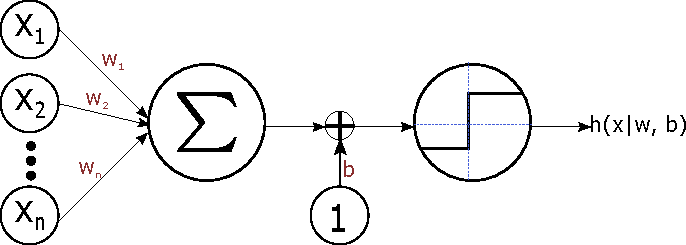
\includegraphics[width=0.8\textwidth]{perceptron.pdf}
    \caption{The Perceptron}
    \label{fig:perceptron}
\end{figure}
%
This neuron in a human brain corresponds to a perceptron in the computational model. It is composed of $n_{in}$ inputs $\boldsymbol{x} = \{ x_1, ... x_{n_{in}} \}$, $n_{in}$ weights $\boldsymbol{w}$ and a bias $b$. Figure \ref{fig:perceptron} illustrates the working principle of a perceptron. When a perceptron received an input vector $\boldsymbol{x}$, a weighted sum of this vector is performed. If its result is higher than the threshold (controlled by $b$), the perceptron is \textquote{activated} and its output becomes a non-zero value.
Equation \ref{eq:perceptron} represents the mathematical formula of the perceptron where $h$ is the activation function of the formula developed in Equation \ref{eq:step} \cite{matteucci_artificial_2019}.
%
\begin{equation}
    h ( \boldsymbol{x} | \boldsymbol{w}, b) = h \left( \sum^{n_{in}}_{i=1} x_i \cdot w_i + b \right) = h \left( \boldsymbol{w}^{T} \cdot \boldsymbol{x} + b \right)
    \label{eq:perceptron}
\end{equation}
%
\begin{equation}
    h ( \boldsymbol{w}^{T} \cdot \boldsymbol{x} + b) = \begin{cases} 1, & \mbox{if } \boldsymbol{w}^{T} \cdot \boldsymbol{x} + b > 0 \\ 0, & \mbox{Otherwise} \end{cases}
    \label{eq:step}
\end{equation}

As the perceptron performs a weighted sum, those weights can be learned to perform a task of interest. However, this model is limited by the functions it can achieve. In Section \ref{subs:fcl}, we discover how we can use multiple perceptrons to create a \textbf{fully-connected layer} to learn more complex functions.
